\documentclass[11pt]{article}
\usepackage[a4paper,margin=22mm,headheight=16pt]{geometry}
\usepackage{fontspec,xeCJK,xcolor,graphicx,enumitem,fancyhdr,titlesec}
\usepackage{hyperref}
\IfFontExistsTF{Times New Roman}{\setmainfont{Times New Roman}}{\setmainfont{TeX Gyre Termes}}
\IfFontExistsTF{FangSong}{\setCJKmainfont[AutoFakeBold=2]{FangSong}}{\IfFontExistsTF{仿宋}{\setCJKmainfont[AutoFakeBold=2]{仿宋}}{\IfFontExistsTF{FandolFang-Regular.otf}{\setCJKmainfont[AutoFakeBold=2]{FandolFang-Regular.otf}}{\setCJKmainfont{FandolSong-Regular.otf}}}}
\definecolor{ink}{HTML}{173747}\definecolor{accent}{HTML}{227E82}
\hypersetup{colorlinks=true,urlcolor=accent,linkcolor=accent}
\linespread{1.22}\setlength{\parindent}{0pt}\setlength{\parskip}{6pt}
\setlist[itemize]{leftmargin=1.4em,itemsep=3pt}
\titleformat{\section}{\large\bfseries\color{ink}}{}{0pt}{}
\titlespacing*{\section}{0pt}{14pt}{7pt}
\pagestyle{fancy}\fancyhf{}\lhead{\small OMNI LEARNING / 学习手册}\rhead{\small Source-grounded learning}\cfoot{\small\thepage}
\emergencystretch=2em\widowpenalty=10000\clubpenalty=10000
\newcommand{\Needspace}[1]{\par\begingroup\dimen0=#1\relax\vskip0pt plus\dimen0\penalty-100\vskip0pt plus-\dimen0\vskip\dimen0\penalty9999\vskip-\dimen0\vskip0pt\endgroup}
\begin{document}


{\LARGE\bfseries\color{ink} 科学证据与工程取舍}\par

2026-10-08 | Day02/30 | 阅读 8 分钟 + 练习 3 分钟\par\vspace{6pt}

\Needspace{5\baselineskip}\section*{今日导航}

今天回答：一次成功演示，能否证明一项技术已经可用？目标是区分科学解释、工程方案和产品证据。先用一分钟回忆昨日系统拆解：如果只观察到系统成功一次，你还不知道哪些条件？阅读与读图约八分钟，练习三分钟。

\Needspace{5\baselineskip}\section*{从演示走向可检验的问题}

设想一个团队演示桥梁模型承重：放上一个砝码，桥没有倒。这个结果支持的是“在此次条件下承受了这一载荷”，并不自动支持“适合所有地形、能用五十年”。工程判断需要材料、结构、环境与使用条件。OpenStax 把物理学中的模型与实验联系起来；本课把这种证据意识迁移到日常技术阅读。[S1]

\begin{center}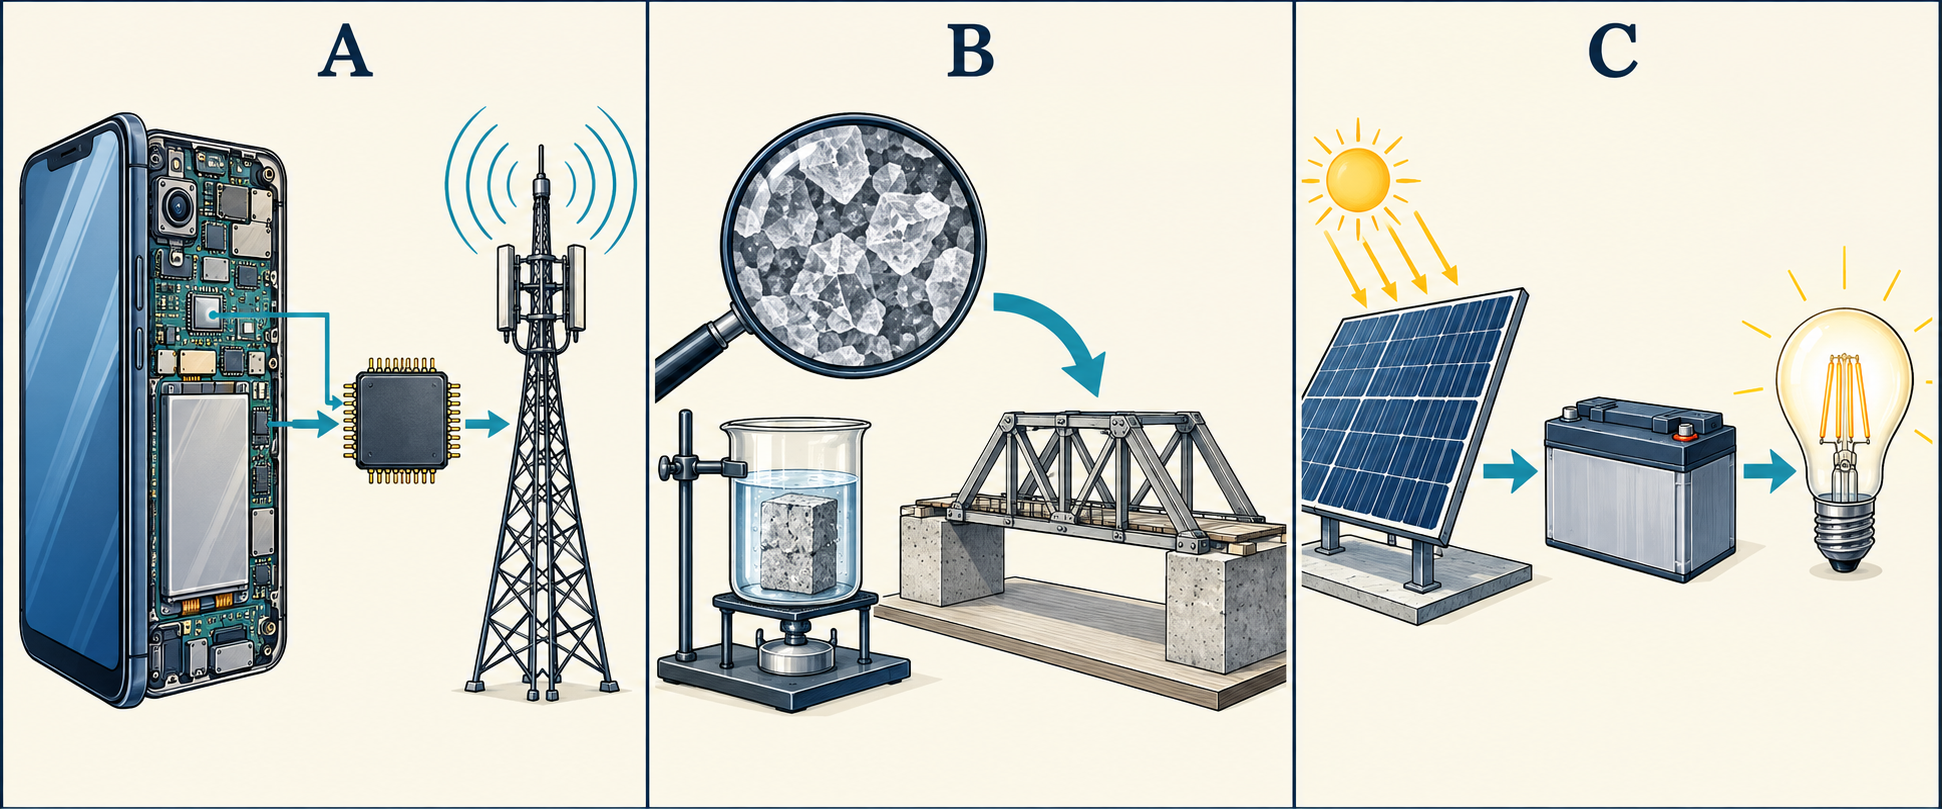
\includegraphics[width=\linewidth,height=0.26\textheight,keepaspectratio]{../assets/figure-f1c69576c177.png}\par

{\small 本课重点看 B 区。A 用手机观察部件与网络；B 区分解释与设计；C 追踪太阳能、储能和照明之间的能量流。箭头为概念关系，不是接线图。}\par

{\footnotesize AI生成教学示意，非实物照片、原始史料或官方架构。生成方式：内置文生图；提示词见仓库 docs/image-prompts.json。}\end{center}

\Needspace{5\baselineskip}\section*{科学问题与工程问题}

科学问题试图解释或预测现象，例如温度变化怎样影响材料。一个可检验的说法要说明观察对象、条件与预期结果。工程问题则问：在预算、寿命、施工和安全约束下，怎样造出符合用途的结构？同一原理可以导向不同设计，设计也可能为了成本牺牲部分性能。

因此“原理成立”“原型能工作”和“批量交付可靠”是三个需要不同证据的阶段。实验室里控制环境有助于识别机制；真实环境的噪声和差异则检验方案是否稳健。不要把早期结果贬为无用，也不要把早期结果直接扩大成成熟产品的承诺。

\Needspace{5\baselineskip}\section*{如何读一个测试结果}

先问基线：它比什么好？再问条件：样本、任务和环境是什么？然后问指标：平均速度是否掩盖了少量特别慢的情况？最后问代价：性能增加是否带来能耗、成本或维护要求？NIST 的 AI 测量资料列出可靠性、可解释性等维度，可帮助你想到单项准确率以外的问题。[S4]

看图 B：材料观察和桥梁设计之间有联系，但没有一条“观察到原理，所以工程必然成功”的捷径。假设某导航系统在晴天主干道表现良好，评估还应有雨天、复杂路口、定位中断等与用途相关的条件。这些是课程提出的测试建议，不是对某品牌的测试结果。

\Needspace{5\baselineskip}\section*{三分钟练习：改写宣传句}

原句：“我们的识别系统准确率很高，因此可以替代人工。”请把它改成三个能核实的问题，并写出一个人工保留点。

参考问题：准确率基于哪类样本？漏判与误判分别多少？上线环境是否接近测试环境？人工保留点可以是置信不足或后果严重时的复核。若你的问题只剩“有没有论文”，还不够；有论文也要看方法是否支持具体使用场景。为节省时间，只写问题，不要求今天真的开展测试。

\Needspace{5\baselineskip}\section*{复盘与明日连接}

科学解释帮助理解为什么，工程设计处理约束，产品验收检验目标是否达成。你可以在一条新闻旁写下“已证明什么／还没证明什么”，避免从演示跨越到普遍承诺。明天用能量转换学习另一种限制：有些代价无法仅靠软件更新消失。

\Needspace{6\baselineskip}\section*{扩展学习 / Further reading}\small 以下为选读，不计入每日必做时间。\begin{enumerate}[leftmargin=1.6em]

\item [S1] \href{https://openstax.org/books/physics/pages/1-1-physics-definitions-and-applications}{Physics: Definitions and Applications} — 从物理学与技术的关系入手，区分解释自然和解决实际问题。\par OpenStax | 发布：未标注 | 核验：2026-10-08

\item [S2] \href{https://science.nasa.gov/ems/}{The Electromagnetic Spectrum} — 查看波谱教学材料，理解通信与成像共享的物理基础。\par NASA | 发布：未标注 | 核验：2026-10-08

\item [S3] \href{https://www.energy.gov/oe/electricity-101}{Electricity 101} — 只读发电、输电、配电与 kWh 的基础解释；历史统计不作当前数据。\par 美国能源部 | 发布：未标注 | 核验：2026-10-08

\item [S4] \href{https://www.nist.gov/ai-measurement-and-evaluation}{AI measurement and evaluation} — 观察准确性之外的可靠性与可解释性维度，为后续技术评估做准备。\par NIST | 发布：未标注 | 核验：2026-10-08

\item [S5] \href{https://www.computerhistory.org/siliconengine/}{The Silicon Engine} — 沿晶体管与集成电路历史观察技术如何通过多项改进进入系统。\par Computer History Museum | 发布：未标注 | 核验：2026-10-08

\end{enumerate}

\end{document}